% \documentclass[10pt,executive]{article}
% \usepackage[left=1in,top=1in,right=1in,head=1in,foot=1in]{geometry}
% \usepackage{times}
% \usepackage{setspace}
% % \usepackage{fancyhdr}
% % \usepackage[yyyymmdd,hhmmss]{datetime}
% % \pagestyle{fancy}
% % \rfoot{Compiled on \today\ at \currenttime}
% % \cfoot{}
% % \lfoot{Page \thepage}
% 
% \linespread{1.0}
% \usepackage{graphicx}
% \usepackage{booktabs}
% % \usepackage{multibbl}
% \usepackage{amsfonts,amssymb,pxfonts}
% \usepackage{mathrsfs}
% \usepackage{epsfig}
% \usepackage{latexsym}
% \usepackage{algorithm}
% % \usepackage{amsmath}
% \usepackage{algorithmic}
% \usepackage{appendix}
% \usepackage{color}
%  
% % \usepackage[belowskip=-8pt,aboveskip=0pt]{caption}
% \usepackage{changepage}
% \usepackage{url}
% 
% \usepackage{multibib}
% \newcites{pri}{Primary sources}
% \newcites{sec}{Secondary sources}

\documentclass[a4paper,8pt]{article}

\usepackage{a4wide}
%\usepackage{a4extrawide}
%\usepackage[latin1]{inputenc}
\usepackage[utf8]{inputenc}
\usepackage[T1]{fontenc}
\usepackage{graphics}
%\usepackage{graphicx}
\usepackage{graphicx,rotating,booktabs}
\usepackage{hyperref}
\usepackage[strings]{underscore}
\usepackage{amssymb}
\usepackage{eurosym}
\usepackage{xspace}
% \usepackage{multibib}
\usepackage{todonotes}
\usepackage{enumitem}
\usepackage{caption}
\usepackage{colortbl}
\usepackage[compact]{titlesec}
\usepackage{setspace}


\DeclareMathSymbol{\varPi}{\mathord}{letters}{"05}





\newcommand{\noop}[1] {}
\newcommand*{\QEDA}{\hfill\ensuremath{\blacksquare}}
\newcommand*{\QEDB}{\hfill\ensuremath{\square}}

\newtheorem{definition}{\bf Definition}
% \newtheorem{proof}{\bf Proof}
%  \newtheorem{definition}{\bf Definition}
%  \newtheorem{theorem}{\bf Theorem}
%  \newtheorem{example}{\bf Example}
% \newtheorem{lemma}{\bf Lemma}
% \newtheorem{corollary}{\bf Corollary}
% \newtheorem{construction}{\bf Construction}
% \renewcommand{\algorithmicrequire}{\textbf{Inputs:}}
% \renewcommand{\algorithmicensure}{\textbf{Outputs:}}
% \renewcommand{\algorithmicensures}{\textbf{Output:}}
\usepackage{xcolor}
\usepackage[scaled=0.85]{helvet}
\renewcommand{\familydefault}{\sfdefault}
\renewcommand{\shapedefault}{n}


% \usepackage{colortbl}
% Flag for showing/suppressing intermediate remarks
\newif\ifTDraft
\TDrafttrue
\let\thesisFinal\TDraftfalse
\let\thesisDraft\TDrafttrue

\newcommand{\DOUBT}[2]{\ifTDraft{\marginpar{\small\em
			\color{red}#2}{\color{blue}#1}}\else#1\fi}
\newcommand{\NB}[2]{\ifTDraft{%
		{\color{red}$\langle\langle$\color{gray}#1\color{red}$\rangle\rangle$}%
		{\color{blue}$\langle\langle$\color{gray}#2\color{blue}$\rangle\rangle
			$}%
	}\else#2\fi}
\newcommand{\NEW}[1]{\ifTDraft{\color{blue}#1}\else#1\fi}
\newcommand{\CUT}[1]{\ifTDraft{\color{red}#1}\else{}\fi}
\newcommand{\CHG}[2]{\ifTDraft{{\color{red}#1}{\color{blue}#2}}\else#2
	\fi}



%%%%%%%%%%%%%%%%%%%%%%%%%%%%%%%%%%%%%%%%%%%%%%%%%%%%%%%%%%%%%%%%OLD%%%%%%%%%%%%%%%%%%%%%%%%%%%%
\begin{document}
	
	\title{Formalism and Paradigm}
	\maketitle

% =============================================================================================
\tableofcontents

~\newpage
% =============================================================================================
\section{Introduction}	


\begin{figure}[h]
\centering
\begin{center}
 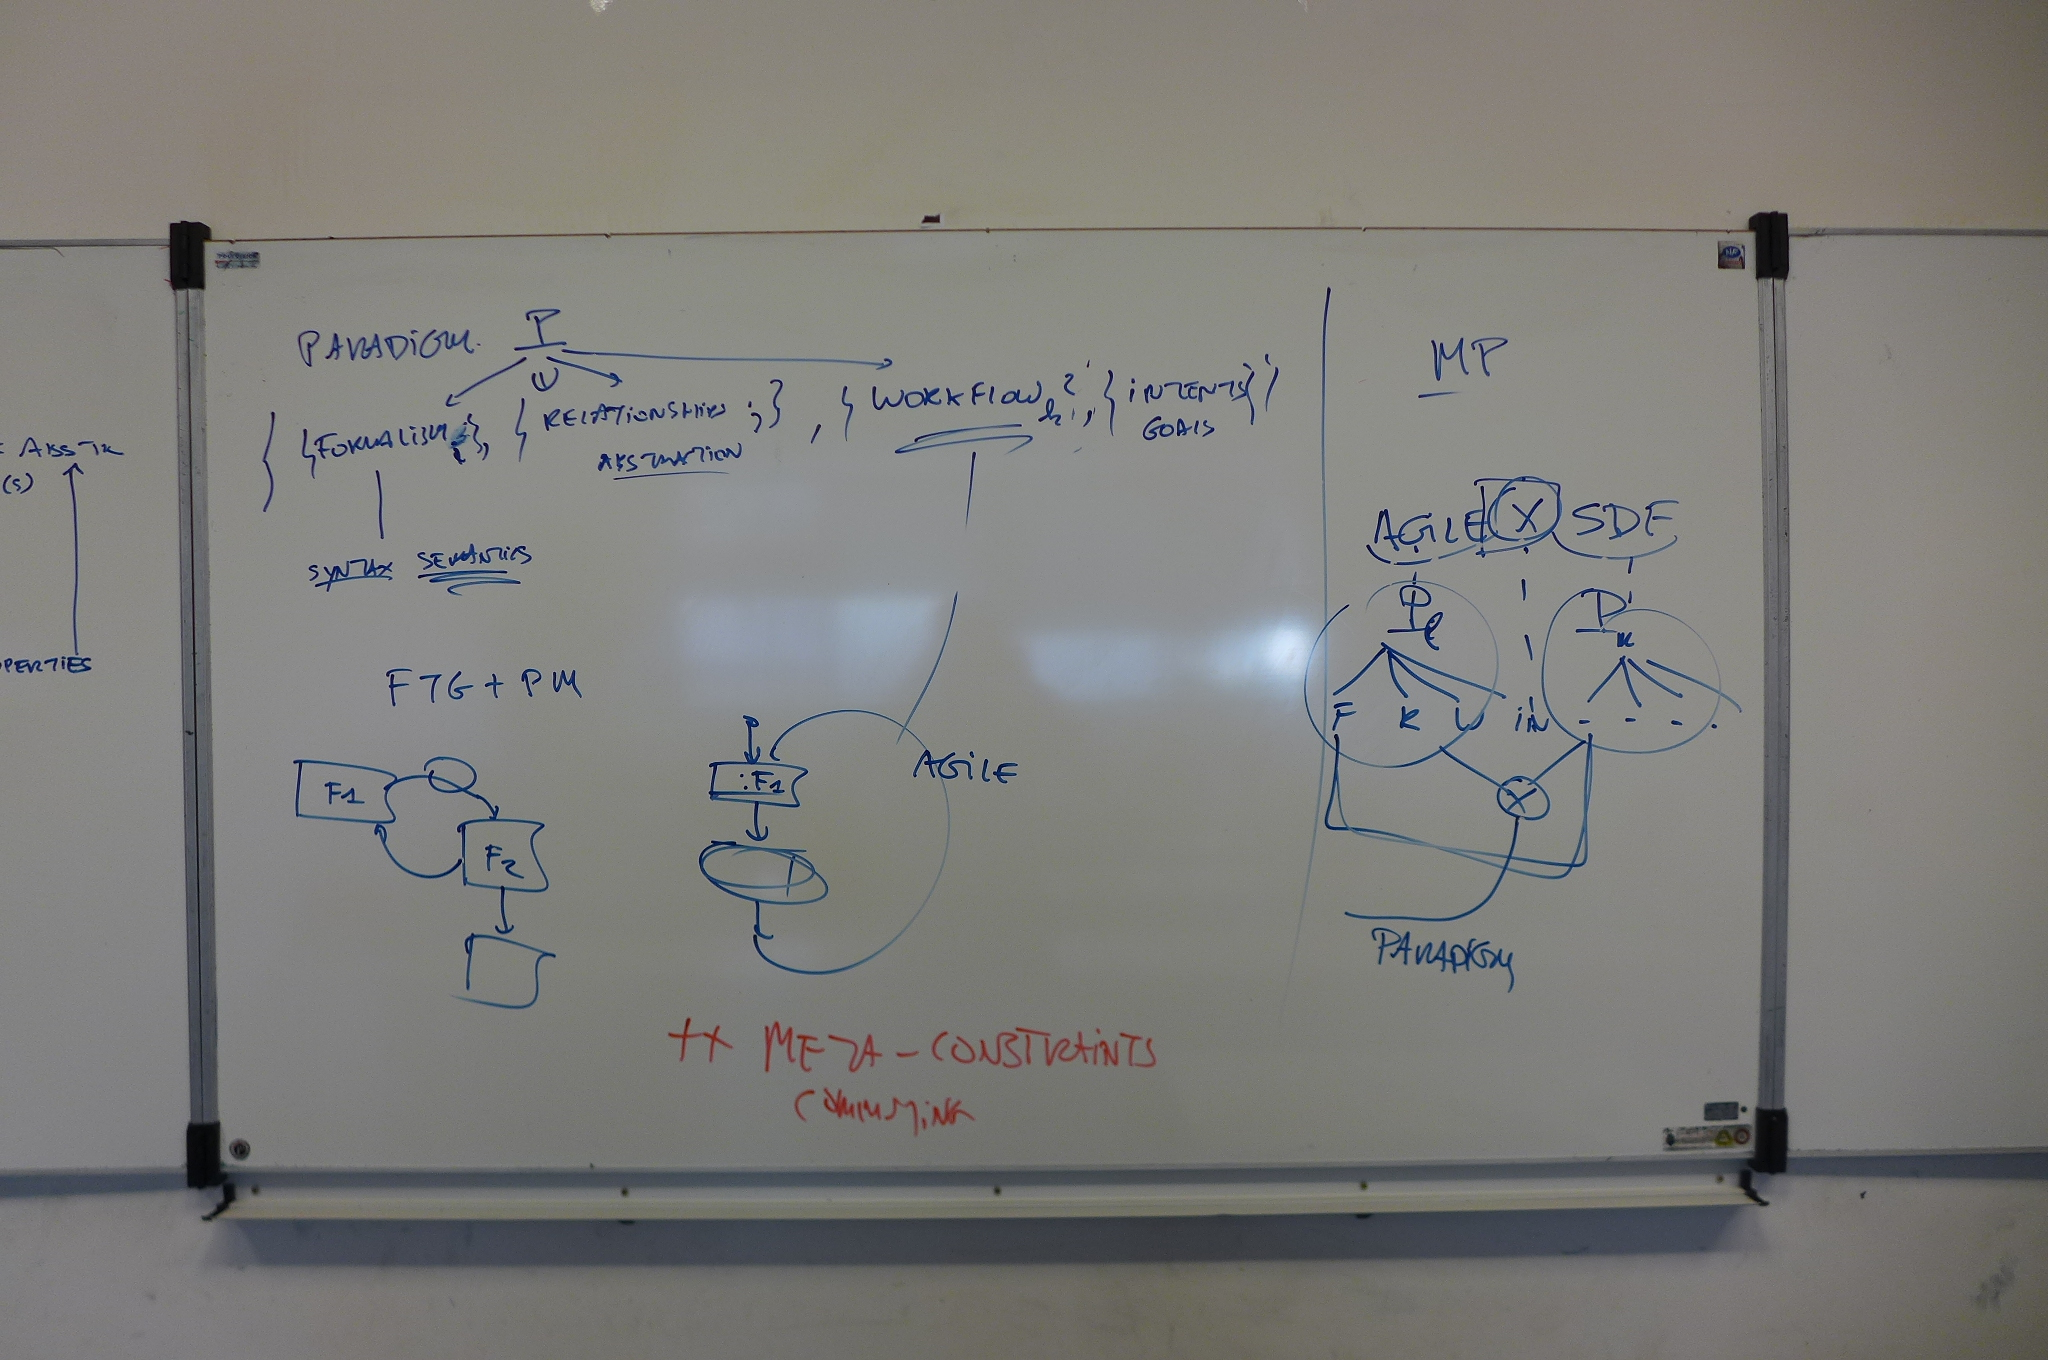
\includegraphics[scale=0.50]{P1130927.jpg}
\caption{Multi-Paradigm Def. from Hans}
\label{fig:paradigm-hans}
\end{center}
\end{figure}
%  

remark: paradigm in Figure~\ref{fig:paradigm-hans} is named multi-paradigm approach here

reason: otherwise multi-paradigm would require to combine workflows, intent, relations and formalisms (which I think is not always the case)




% =============================================================================================
\section{(Modeling) Paradigms}	

TODO: use Matlab/Simulink without stateflow and simulation as example


\subsection{(Modeling) Paradigm}	

\begin{definition}[(modeling) paradigm]
An \emph{(modeling) paradigm} is a set of modeling formalisms, relations between models, modeling scenarios, and modeling intents employed to develop systems.
\end{definition}
\todo[inline]{ add ontology fragment for this definition }

modeling intents is meant in a broad sense including analysis steps such as simulation etc.

My understanding is that an extension/generalisation of the Software Manufacture Models and its notion of  Software Manufacture Model Patterns from \cite{HebigPhD2014} would be helpful here.
\todo[inline]{
see 
Figure 6.12.: Meta model of Software Manufacture Model language​
and
Figure 6.22.: Meta model of Software Manufacture Model Pattern language​
}
%
% HebigPhD2014:
% Regina Hebig. Evolution of model-driven engineering settings in practice. PhD thesis, Hasso-Plattner-Institut fur Softwaresystemtechnik, Universität Potsdam, 2014.
% https://www.hpi.uni-potsdam.de/giese/bibadmin/show.php?id=13631​
%
% see uploaded HebigPhD2014.pdf

\todo[inline]{
ADDED: 

- add \emph{relational view} for a paradigm $=$ relations between these models

- add \emph{workflow} offered by each paradigms $=$ modeling scenarios (maybe workflow/process fragments); mega models and mega model fragments can be employed to describe approaches (see Regina Hebig's work)

- add \emph{intents/goals} supported by a paradigm $=$ modeling intents

BUT: here emphasis is on the combination at the level of the formalisms!


STILL to be ADDED: 

- scenario may employs part of the \emph{workflow} offered by each paradigms to realize a new partial workflow (e.g., offer a worlfow to do a simulation for the joint models that employs steps of workflows for simulate the separate models)

- combine \emph{intents/goals} supported by each paradigms (e.g, allow validation of a combined view based on the validation capabilities for each paradigm on its own)

- combine \emph{relational view} elements offered by each paradigms into joint \emph{relational view} elements (e.g, allow optimization of a combined view for criteria provided for each paradigm or criteria for thier combination)

}


\subsection{(Modeling) Formalism}

EXAMPLE: Matlab/Simulink without stateflow

\subsection{(Modeling) Relations}

EXAMPLE: ???

\subsection{(Modeling) Scenario}


\begin{definition}[(modeling) scenario]
A \emph{scenario} is a setup that support one or multiple activities, employs one or multiple models and their employed formalisms as inputs or outputs, and employs tools or model composition of the formalisms for the activities. 
\end{definition}
\todo[inline]{ add ontology fragment for this definition }

\todo{ HG: mega model fragments can be employed to describe such scenarios }

\todo{ HG: We may use the HPI Lab example to clarify the terms? }


EXAMPLE: Simulation of a Matlab/Simulink model and subsequent adjustments


\subsection{(Modeling) Intents}


EXAMPLE: intent is to ensure the proper control behavior of the Matlab/Simulink model 

\subsection{Special Cases}

- \emph{single-formalism paradigm} is a paradigm employing only a single formalism

- \emph{multi-formalism paradigm} is a paradigm employing multiple formalisms



% =============================================================================================
\section{Cyber-Physcial System \& (Modeling) Paradigms}	

\section{Cyber-Physical System Development}

In case of cyber-physical systems, models and their employed formalisms can be employed to capture fragments of the cyber and the physical part of the overall systems. Accordingly, we name a multi-paradigm scenario cyber-physcial if both kinds of fragments are covered. 

\subsection{Cyber-Physical Scenario}

\begin{definition}[cyber-physical scenario]
A \emph{cyber-physical scenario} is a scenario where the models and their employed formalisms capture fragments of both the cyber and  physical parts of an overall systems. 
\end{definition}
\todo[inline]{ add ontology fragment for this definition }



% =============================================================================================
\section{Multi-Paradigm Modeling}

- \emph{multi-paradigm} is a combination of paradigms, but as we will see the combination can be achieved quite differently

	

\begin{figure}[h]
\centering
\begin{center}
 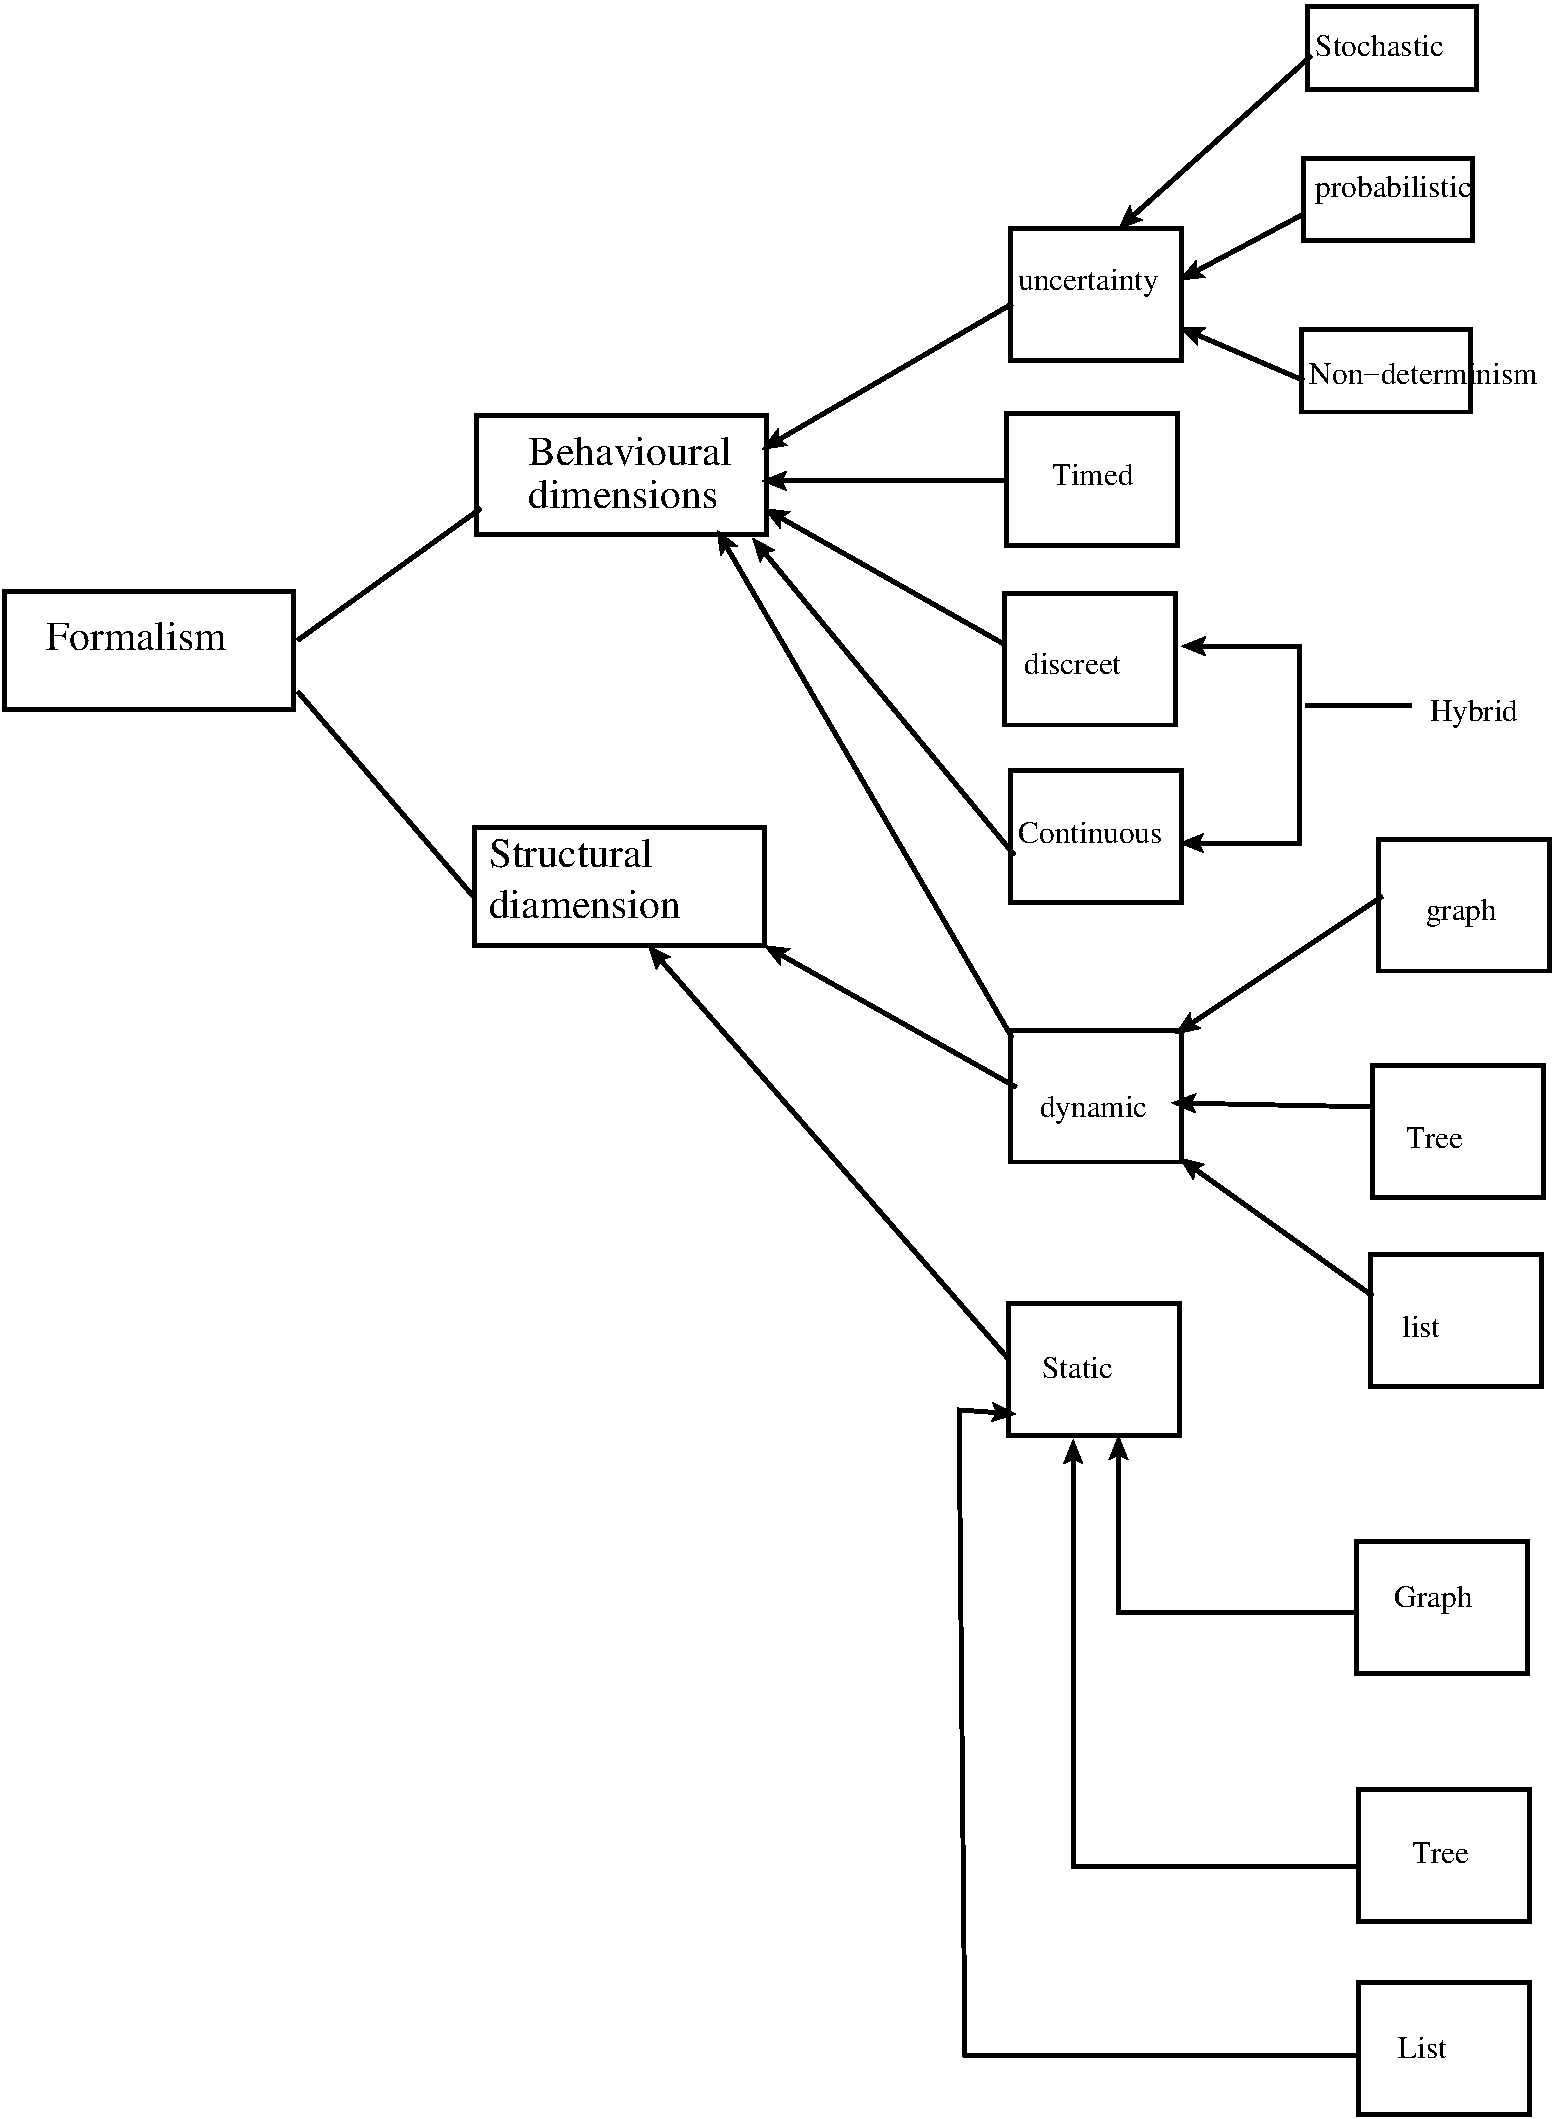
\includegraphics[scale=0.25]{overview}
\caption{Overall overview in schematic format}
\label{fig:arch}
\end{center}
\end{figure}
\todo{\small HG for SB: replace errors by UML generalization; replace Formalism by Paradigm; replace dynamic by dynamic structure; static by  static structure}
%  
In Figure~\ref{fig:arch} the most basic features of a paradigm are outlined. We at first have a \emph{behavioral dimension} and \emph{structural dimension}. For each dimension we have distinguishable \emph{features} that a paradigm can support. Both dimension can also be subsequently combined in form of the \emph{dynamic structure} feature. \todo[inline]{...}


\subsection{Multi-Paradigm (Modeling)}
%
As outlined in Figure~\ref{fig:arch}, a paradigm could cover different dimensions of a system to a different extent (covering only a subset of the possible features). 
%
\begin{definition}[relations between paradigms, core paradigm, multi-paradigm]
A paradigm can support the different dimensions of systems to such an extent that it \emph{conceptually equals} another paradigm when it supports for the same dimensions exactly the same features. 
%
A paradigm can support the different dimensions of systems to such an extent that it \emph{conceptually includes} another paradigm when it supports all features of all  dimensions that the other paradigm supports and is not equal. 
%
A paradigm can support the different dimensions of systems to such an extent that it \emph{conceptually different} from another paradigm when it supports different dimensions or different features for the same dimension. 
%
A \emph{core paradigm} is then a paradigm that is not a conceptual extension of another paradigm (it does not exists a paradigm it conceptually includes).
%
A \emph{multi-paradigm} is then a paradigm that does conceptual include multiple core paradigms.
%
\end{definition}
\todo[inline]{ add ontology fragment for this definition }

IMPORTANT: It seems that a multi-paradigm does not necessarily support all relations, scenarios, and intents of a conceptually included or conceptually equal one.



For example, the ODE (ordinary differential equation) paradigm is a single-formalism paradigm and a core paradigm that captures only the continuous and timed behaviour features of the behavior dimension, but not the discrete behavior feature,
%
the automata paradigm is a single-formalism paradigm and a core paradigm that captures only the discrete feature of the behavior dimension, but not the continuous and timed behaviour features, and
%
the hybrid automata paradigm is a single-formalism paradigm and a multi-paradigm, as it employs only one formalism but includes the automata and ODEs paradigms and their features of discrete, continuous, and timed behaviour for the behavior dimension. 


In contrast, the Simulink/Stateflow paradigm is a multi-formalism paradigm and a multi-paradigm, as it employs both the Simulink and Stateflow formalism and includes the Simulink and Stateflow paradigms that are conceptually similar to ODEs and automata.




% ==========================================================================================
\subsection{Forms of Multi-Paradigm Scenarios}
%
Given formalisms supporting paradigms, multi-paradigm scenarios can operate in three different ways:
%
\begin{itemize}
 \item Language-based: Having a single-formalism paradigm that includes multiple core paradigms (e.g., hybrid automata)
 \item Composition-based: We compose formalism supporting different paradigms into a single one by a suitable model of computation that composes the multiple formalisms (e.g., Simulink/Stateflow)
 \item Tool-based: We compose formalisms supporting different paradigms via tools (e.g., co-simulation of a Simulink model and a plant model)
\end{itemize}

\begin{definition}[multi-paradigm scenario]
A \emph{multi-paradigm scenario} is a scenario which covers parts of scenarios from at least two core paradigms. 

\todo[inline]{ HG: add the three cases to definition? }

\end{definition}
\todo[inline]{ add ontology fragment for this definition }


EXAMPLE: simulation

% =======================================================================================
\subsubsection{Examples for Language-based Multi-Paradigm Scenarios}

Hybrid automata

HGTS


\begin{figure}[h]
\centering
\begin{center}
 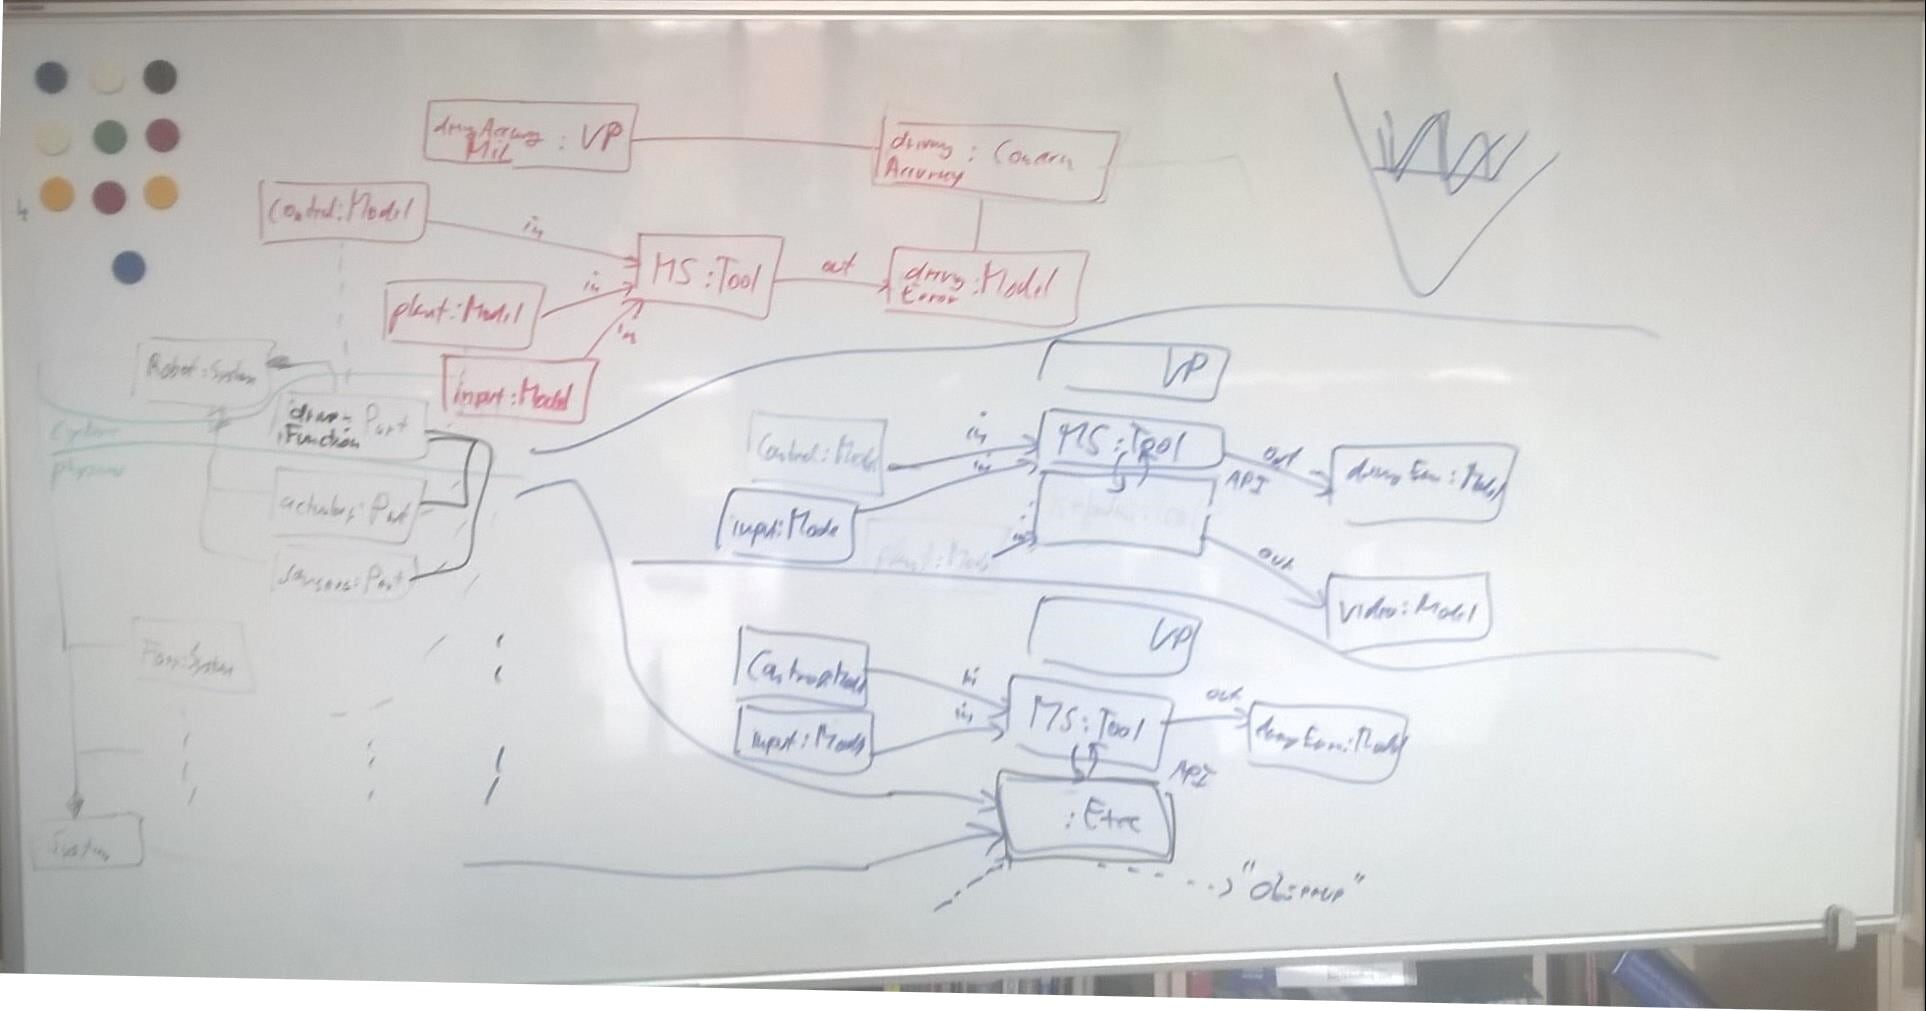
\includegraphics[scale=0.25]{hpi_cps_lab_viewpoints_1.jpg}}
\caption{HPI-CPS Lab View-1}
\label{fig:view1}
\end{center}
\end{figure}


Matlab/Simulink with Stateflow (see Figure~\ref{fig:view1} top, where the different models employing stateflow for the software and Simulink for the plant are supported as a multi-formalism and simulated jointly)

...

	
% =======================================================================================
\subsubsection{Examples for Composition-based Multi-Paradigm Scenarios}

Ptolemy

https://ptolemy.berkeley.edu/

Ptolemy II

ptolemy.berkeley.edu/ptolemyII/


\begin{figure}[h]
\centering
\begin{center}
 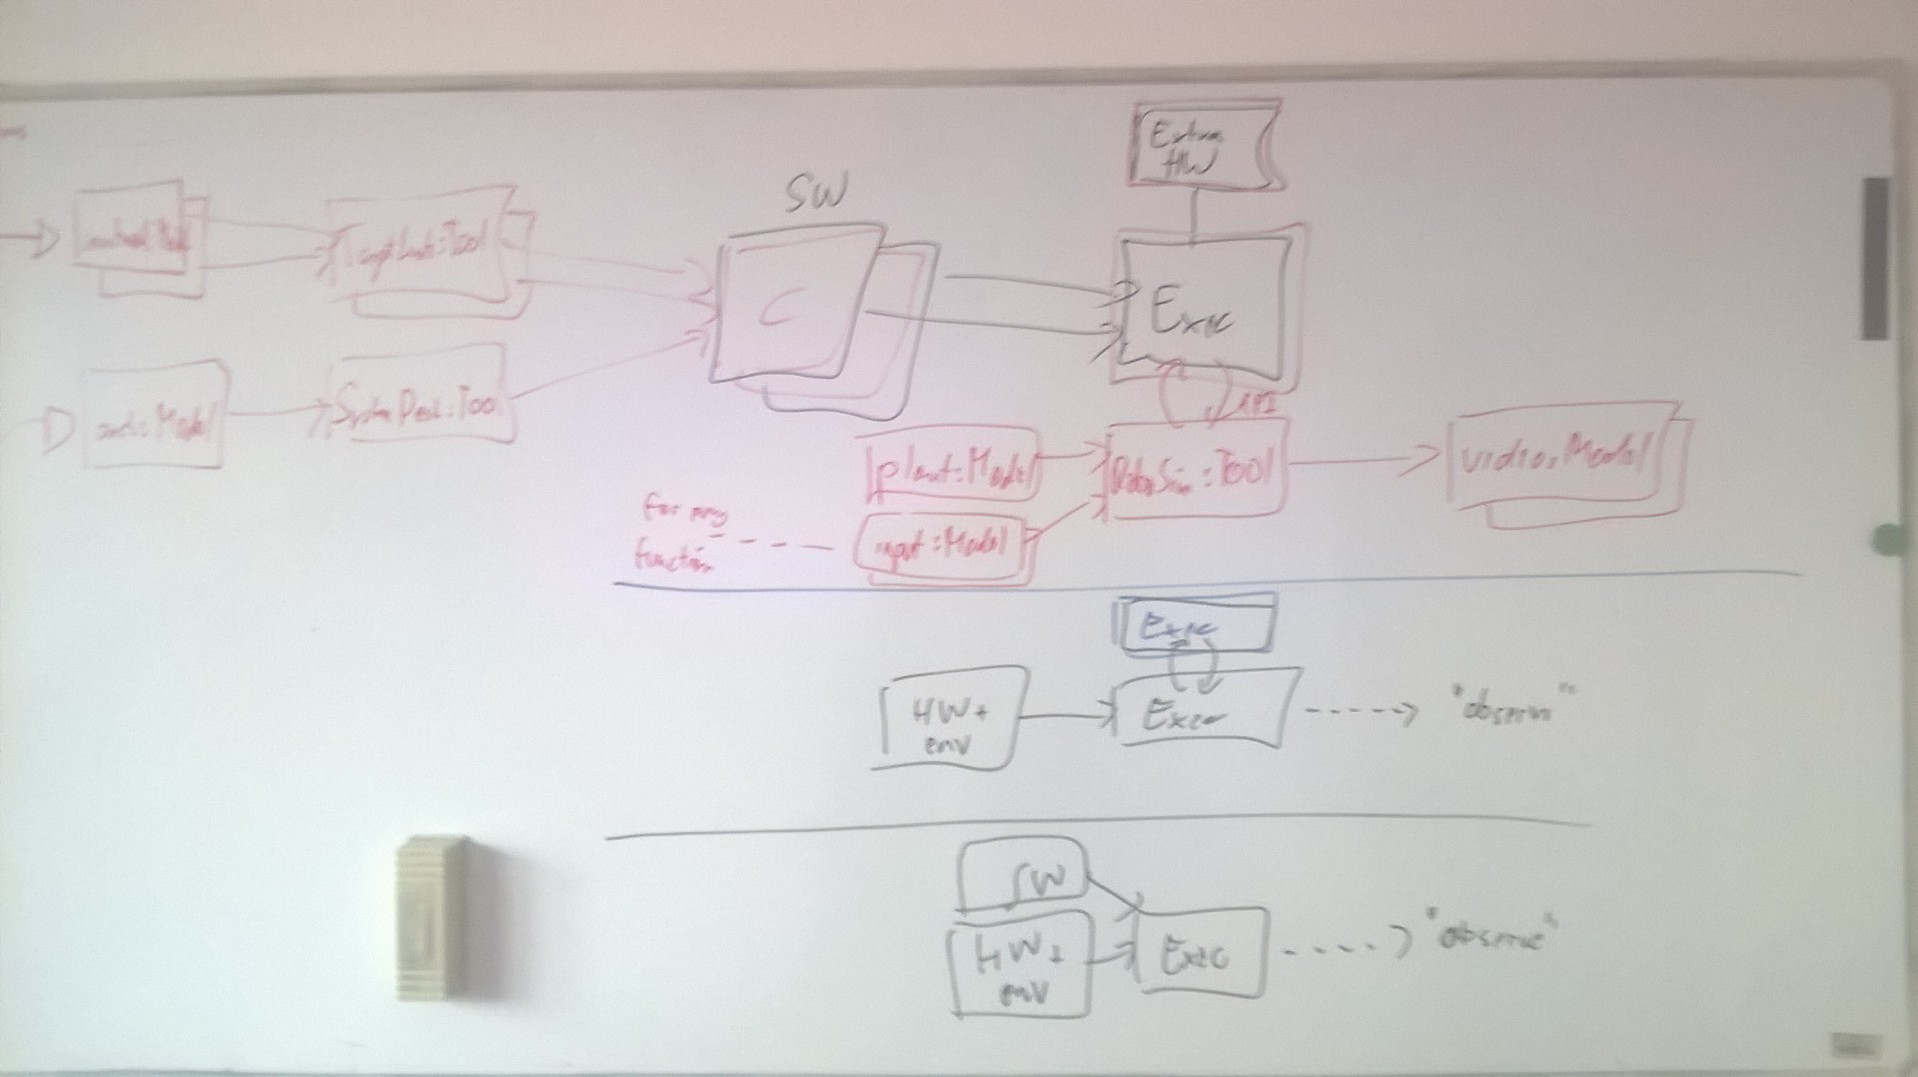
\includegraphics[scale=0.25]{hpi_cps_lab_viewpoints_2.jpg}}
\caption{HPI-CPS Lab View-2}
\label{fig:view2}
\end{center}
\end{figure}


Matlab/Simulink with Stateflow for the software functions and AUTOSAR SystemDesk for the software architecture build a multi-formalism coupling that is resolved by linking the generated c-code and executed together with a simulator of the plant (see Figure~\ref{fig:view2} top, where the coupled via coupling of software execution and simulator for the plant).



% ========================================================================================
\subsubsection{Examples for Tool-based Multi-Paradigm Scenarios}


Matlab/Simulink with Stateflow for the software and a configuration for RoboSim are coupled via co-simulation (see Figure~\ref{fig:view1} middle, where the models are coupled via coupling of the Matlab/Simulink and RoboSim simulators).


Matlab/Simulink with Stateflow for the software and Robot as rapid prototype can also be coupled by linking the Matlab/Simulink simulator with the execution of the robot (see Figure~\ref{fig:view1} bottom: coupled via coupling of simulator and robot (exec)).



Matlab/Simulink with Stateflow for the software functions and AUTOSAR SystemDesk for the software architecture build a multi-formalism coupling that is resolved by linking the generated c-code and executed together with a rapid prototype of the plant (see Figure~\ref{fig:view2} middle, where the execution of the software is coupled with a robot).


final outcome where all is mapped to the execution on one host:

Matlab/Simulink with Stateflow for the software functions and AUTOSAR SystemDesk for the software architecture build a multi-formalism coupling that is resolved by linking the generated c-code and executed together with a rapid prototype of the plant (see Figure~\ref{fig:view2} bottom, where the execution of the software is done on the robot).



% =============================================================================================
\section{Cyber-Physical Multi-Paradigm Modeling}

cyber-physical system can be modelled with multi-paradigm

\todo[inline]{Incomplete sentence}

\begin{definition}[cyber-physical multi-paradigm scenario]
A \emph{cyber-physical multi-paradigm scenario} is a multi-paradigm scenario where the models and their employed formalisms capture fragments of both the cyber and  physical parts of an overall systems. 
\end{definition}
\todo[inline]{ add ontology fragment for this definition }

As the cyber and physcial domains usually require specific paradigms usually/often cyber-physical scenario are also cyber-physical multi-paradigm scenarios.


\subsection{Cyber-Physical Multi-Paradigm}

\begin{definition}[cyber-physical multi-paradigm]
A \emph{cyber-physical multi-paradigm} is a multi-paradigm capable of covering physical as well as cyber apsectsfor the development.
\end{definition}
\todo[inline]{ add ontology fragment for this definition }


% =============================================================================================
\section{Example}
\todo{HG: move to the definitions?}

\todo[inline]{
Here we should start with a copy of Section ''6.2 HPI CPS Lab'' from ''fw_combine_modeling_languages'' (including the figures!)
}

% =============================================================================================
\section{Existing Paradigms \& Multi-Paradigms}

% ==========================================================================================
\subsection{Single-Formalism Paradigms}


Through Table \ref{tab:existing-model} and \ref{tab:existing-models}, we have characterized the formal model.	

	\newcommand{\HC}{\cellcolor[gray]{0.8}}
	
	\begin{table}[ht]
		\centering
		\caption{Existing/planned models, their dimension and tool support.
			We have characterized our model under a common underlying modeling  paradigm.
			(1) (GTS) Graph Transformation System: Under this category the following models have been depicted
			Normal GTS, (TGTS) Timed Graph Transformation System, (HGTS) Hybrid graph transformation systems;
			(2) Under process algebra:
			(BPA) Basic process algebra: (RT) Rewrite Theory, $\pi$ calculus, (RTRT) Real-Time Rewrite Theory, (TBPA) Timed basic process algebra;
			(3) Under Petri net (PN): Ordinary PN, (TPN) Time Petri net, (HPN) Hybrid Petri net; 
			(4) Under automata based model: (TA) Timed Automaton,(HA) Hybrid automata;(HBG) Hybrid Bond Graph.
			%(5) Under combined model: MsC) Message sequence chart, (Event B) Event B systems,  
			\textbf{Structure~dimension:} is divided in to two parts (1) Static and (2) Dynamic  and each part has been divided in to three category (1) Tree, (2) Graph and (3) List;
			Grey color \HC (++) : cover with adaptation, $\times$: not covered at all; 
			\textbf{Behavio dimension:}  is divided in to three category (1) Timed , (2) Discreet and (3) Continuous 
			$\times$ ~none, Grey color (++) ~covered;
			\textbf{Uncertainty:} Divided into three parts (1) Stochastic (2) non determinism and (3) probabilistic; $\times$ ~none, Grey color (++) ~covered;
			% \textbf{Probabilistic behavior:} (--)~none, (+)~probabilistic, (++)~probabilistic / nondeterministic, (+++)~interval~probabilistic / nondeterministic.
			%  The models and tools in bold face were developed by the applicant 
			% and co-workers. 
			% 
		} 
		\scalebox{0.58}{%
\begin{tabular}{|r||p{1.0cm}|p{1.0cm}|p{1.0cm}|p{1.0cm}|p{1.4cm} |p{1.5cm}|p{1.5cm}|p{1.7cm}|p{1.7cm}| p{1.5cm}|p{1.7cm}|p{1.7cm}||p{3.6cm}|}
\hline
\textbf{Model} & \multicolumn{6}{c|}{\textbf{Structural dimension}} & \multicolumn{6}{|c|}{\textbf{Behavioral dimension}}  & \textbf{Verification tools} \\ \hline
				
			&\multicolumn{3}{c|}{\textbf{Static}} & \multicolumn{3}{c|}{\textbf{Dynamics}} & Time & Discreet & Continuous  & \multicolumn{3}{c|}{\textbf{Uncertainty}} & \\ \hline
% 				
 			& Tree & Graph & List &	 Tree & Graph & List & & & & Stochastic & Non determinism & probabilistic & \\ \hline 
% 			
			
			%	\multicolumn{14}{|c|}{\emph{Existing basic models and their verification techniques}}\\ \hline
% 				\hline
				\multicolumn{14}{|c|}{\emph{Graph Transformation Systems (GTS)}}\\ \hline
% 				
			
			
% 			
			Normal GTS  & \HC (++)  & \HC (++) & $\times$ & \HC (++)  & \HC (++) & $\times$   & $\times$ & $\times$ &  $\times$ & $\times$   & $\times$ & $\times$ &
				AGG~\cite{Taentzer04}, GROOVE~\cite{groove}, \textbf{HENSHIN}~\cite{ABJ+10}, 
				\textsc{Moment}2~\cite{Boronat2009}, \textsc{Viatra}~\cite{viatra}, 
				\textbf{Inductive Invariant Checker} \cite{GSKBB06} \\ \hline
% 				
			
			
			
			TGTS  & \HC (++)  & \HC (++) & $\times$ & \HC (++)  & \HC (++) & $\times$   & \HC (++) & $\times$ &  $\times$ & $\times$   & $\times$ & $\times$ & \textbf{Timed GROOVE}~\cite{Neumann07}, 
				\textsc{Moment}2~\cite{BO10}, \textbf{Inductive Invariant Checker} \cite{GieseBecker08}\\ \hline
				
				
% 				
	HGTS & \HC (++)  & \HC (++) & $\times$ & \HC (++)  & \HC (++) &
 $\times$   & \HC (++) & \HC (++) &  \HC (++)  & $\times$  & $\times$ & $\times$ &  GROOVE~\cite{groove} \\ \hline     
	

				SGTS &  \HC (++) & \HC (++) & $\times$ & \HC (++)  & \HC (++) & $\times$  & \HC (++) & $\times$ & $\times$ & \HC (++)  & $\times$ &  $\times$ & GROOVE + PRISM~\cite{HLM06}, 
				\textbf{HENSHIN} + PRISM~\cite{ABJ+10}, 
				        \textsc{Viatra} + \textsc{GraSS}~\cite{THR10} \\ \hline	


				PGTS &  \HC (++) & \HC (++) & $\times$ & \HC (++)  & \HC (++) & $\times$  & $\times$ & $\times$ & $\times$ & $\times$  & \HC (++) &  \HC (++) & \textbf{HENSHIN} + PRISM~\cite{KG12a}
				 \\ \hline 
% 				
% 				
% 				
% 				
% 				
	\multicolumn{14}{|c|}{\emph{Process Algebra (PA)}}\\ \hline
% 				
% 				
% 				
% 				% 
	BPA &  $\times$ & $\times$ & \HC (++) & $\times$  & $\times$ & \HC (++)  & $\times$ & $\times$ &  $\times$ & $\times$  & $\times$ & $\times$  & TAPA \cite{Calzolai2008}\\ \hline
% 			
			   RTPA & $\times$ & $\times$ & \HC (++) & $\times$  & $\times$ & \HC (++)  & \HC (++) & \HC (++) &  \HC (++) & $\times$  & $\times$ & $\times$  & $\times$ \\ \hline
% 			  
	TBPA & $\times$ & $\times$ & \HC (++) & $\times$  & $\times$ & \HC (++)  & \HC (++) & $\times$ &  $\times$ & $\times$  & $\times$ & $\times$ & MsC generator \cite{msc}         \\ \hline
% 			  
% 			   
			   \multicolumn{14}{|c|}{\emph{Rewriting theory (RT)}}\\ \hline
% 			
% 		    	
				RT   &  $\times$ & $\times$ & \HC (++) & $\times$  & $\times$ & \HC (++)  & $\times$ & $\times$ &  $\times$ & $\times$  & $\times$ & $\times$ &  \textsc{Maude}~\cite{Clavel2002} \\ \hline\hline
% 				
% 				
			RTRT  &  $\times$ & $\times$ & \HC (++) & $\times$  & $\times$ & \HC (++)  & \HC (++)  & \HC (++)  &  \HC (++)  & $\times$  & $\times$ & $\times$ & \textsc{Maude}~\cite{OM07} \\ \hline
% 				
% 				
% 				\multicolumn{10}{|c|}{\emph{Rewriting theory (RT)}}\\ \hline
% 				
				$\pi$ Calculus  &  $\times$ & $\times$ & \HC (++) & $\times$  & $\times$ & \HC (++)  & \HC (++)  & \HC (++)  &  \HC (++)  & $\times$  & $\times$ & $\times$ & Mobility Workbench (MWB) \cite{mwb}\\ \hline
% 				
% 			
% 				
% 			
% 				
% 				
% 				
% 				
				\multicolumn{14}{|c|}{\emph{Petri net (PN)}}\\ \hline
% 				
% 				
% 				
% 				
% 				
	Ordinary PN      &  $\times$ & \HC (++) & \HC (++) & $\times$  & \HC (++) & \HC (++)  & $\times$ & $\times$  &  $\times$  & $\times$  & $\times$ & $\times$ & GHENeSys~\cite{Silva2008}, 
				JFern \cite{jfern},  SamaTulyata\cite{atva}         \\ \hline
% 				
% 				
% 				
				TPN   &  $\times$ & \HC (++) & \HC (++) & $\times$  & \HC (++) & \HC (++)  & \HC (++) & $\times$  &  $\times$  & $\times$  & $\times$ & $\times$ &  CPN \cite{cpn}, Romeo \cite{Gardey2005}         \\ \hline
% 				% 
				HPN  &  $\times$ & \HC (++) & \HC (++) & $\times$  & \HC (++) & \HC (++)  & \HC (++) & \HC (++) &  \HC (++)  & $\times$  & $\times$ & $\times$  & HISIm \cite{hisim}        \\ \hline
% 				
% 				
% 				
% 				
% 				
% 				

%%%%%%END%%%%%%%%%%%%%

			\end{tabular}
			% }
			% \vspace{-1mm}
			
		}
		\label{tab:existing-model}
		% \vspace{-5mm}
	%\end{sidewaystable}

	\end{table}
	
	
	
	
	
	
	
	
	%\newcommand{\HC}{\cellcolor[gray]{0.8}}
	
	\begin{table}[ht]
		\centering
		\caption{We have characterized our model under a common underlying probabilistic modeling  paradigm.
			(1) (DTMC) Discreet time Markov Chain (2) Markov decision process (3) Interval Markov decision process (4) Probabilistic graph transformation systems
			(5) Stochastic graph transformation systems (6) Interval probabilistic timed automata
			. 
			% 
		} 
		\scalebox{0.58}{%
\begin{tabular}{|r||p{1.0cm}|p{1.0cm}|p{1.0cm}|p{1.0cm}|p{1.4cm} |p{1.5cm}|p{1.5cm}|p{1.7cm}|p{1.7cm}| p{1.5cm}|p{1.7cm}|p{1.7cm}||p{3.6cm}|}
\hline
\textbf{Model} & \multicolumn{6}{c|}{\textbf{Structural dimension}} & \multicolumn{6}{|c|}{\textbf{Behavioral dimension}}  & \textbf{Verification tools} \\ \hline
				
			&\multicolumn{3}{c|}{\textbf{Static}} & \multicolumn{3}{c|}{\textbf{Dynamics}} & Time & Discreet & Continuous  & \multicolumn{3}{c|}{\textbf{Uncertainty}} & \\ \hline
% 				
 			& Tree & Graph & List &	 Tree & Graph & List & & & & Stochastic & Non determinism & probabilistic & \\ \hline 
% 			
				

				\multicolumn{14}{|c|}{\emph{Automata and graph based model}}\\ \hline
% 				
% 				
				TA      &  $\times$ & $\times$ & $\times$ & $\times$  & $\times$ &$\times$  & \HC (++) & $\times$ & $\times$  & $\times$  & $\times$ & $\times$  & \textsc{Kronos}~\cite{DOTY96}, \textsc{Rabbit}~\cite{rabbit}, 
				\textsc{RedLib}~\cite{Wang06}, Uppaal~\cite{LPY97} \\ \hline 
% 				
% 				
% 				
				HA        &  $\times$ & $\times$ & $\times$ & $\times$  & $\times$ &$\times$  & \HC (++) & \HC (++) & \HC (++) & $\times$  & $\times$ & $\times$  & HyTech~\cite{henginger}, 
				KeYmaera \cite{Platzer08,0025392}, Checkmate \cite{Chutinan99verificationof}, ForFET \cite{pallabATVA}        \\ \hline
% 				
% 				
% 				
% 				
% 				
% 				
% 				
% 				
% 				
				HBG  &  $\times$ & $\times$ & $\times$ & $\times$  & $\times$ &$\times$  & \HC (++) & \HC (++) & \HC (++) & $\times$  & $\times$ & $\times$  & SAL \cite{sal}         \\ \hline

				 DTMC &  $\times$ & $\times$ & $\times$ & $\times$  & $\times$ &$\times$  & \HC (++) & $\times$ & $\times$ & $\times$  & $\times$ & \HC (++)  
				 & APMC~\cite{Herault06}, MRMC~\cite{KHH+09}, \textsc{PARAM}~\cite{HHWZ10}, 
			 		PRISM~\cite{KNP11} \\ \hline 
				
				MDP  &  $\times$ & $\times$ & $\times$ & $\times$  & $\times$ &$\times$  & $\times$ & $\times$ & $\times$ & $\times$  & \HC (++) &  \HC (++) 
				 & \textsc{LiQuor}~\cite{CB06}, \textsc{Pass}~\cite{HHWZ10b}, PRISM~\cite{KNP11}, 
						\textsc{ProbDiVinE}~\cite{BBC+08}, \textsc{Rapture}~\cite{JDL02} \\ \hline
						
				IMDP &  $\times$ & $\times$ & $\times$ & $\times$  & $\times$ &$\times$  & $\times$ & $\times$ & $\times$ & $\times$  & \HC (++) &  \HC (++) & \textbf{IPTA-PRISM}~\cite{KG11} \\ \hline 
				

				

				        
				IPTA &  $\times$ & $\times$ & $\times$ & $\times$  & $\times$ & $\times$  &  \HC (++) &  \HC (++) &  \HC (++) & $\times$  & \HC (++) &  \HC (++) &  \textbf{IPTA-PRISM}~\cite{KG11} \\ \hline
				%             
				%   % DAE & $\times$ & $\surd$ &  $\surd$ & $\surd$  &$\surd$ & $\times$ &         
				% %  
				%  % CTMC      & (--) & (S)  & (--) & 
				% % 		APMC~\cite{Herault06}, \textsc{Infamy}~\cite{HHWZ09b}, MRMC~\cite{KHH+09},  
				% % 		\prism~\cite{KNP11}, \textsc{Ymer}~\cite{You05} \\ \hline \hline
				% % DTMC      & (--) & (--) & (+) & 
				% % 		APMC~\cite{Herault06}, MRMC~\cite{KHH+09}, \textsc{PARAM}~\cite{HHWZ10}, 
				% % 		\prism~\cite{KNP11} \\ \hline 
				% % MDP       & (--) & (--) & \HC (++) &
				% % 		\textsc{LiQuor}~\cite{CB06}, \textsc{Pass}~\cite{HHWZ10b}, \prism~\cite{KNP11}, 
				% % 		\textsc{ProbDiVinE}~\cite{BBC+08}, \textsc{Rapture}~\cite{JDL02} \\ \hline
				% % IMDP      & (--) & (--) & \HC (+++)  & \textbf{IPTA-\prism}~\cite{KG11} \\ \hline 
				%  \hline
				% \multicolumn{8}{|c|}{\emph{Existing combined models with certain behavior}}\\ \hline
				%  \hline
				% % SGTS  & \HC (++) & (S)  & (--)  & \groove + \prism~\cite{HLM06}, \textbf{\henshin} + \prism~\cite{ABJ+10}, 
				% %         \textsc{Viatra} + \textsc{GraSS}~\cite{THR10} \\ \hline
				
				% % %        \textbf{Timed Story Sequence Diagrams} \cite{Klein&Giese2007} 
				% %         \\ \hline
				% % \textbf{PGTS} & \HC (++) & (--) & \HC (++)  & \textbf{\henshin} + \prism~\cite{KG12a}
				% %         \\ \hline
				
				% 
				
				% 
				
				
				% TBPA & $\surd$ & $\surd$ & $\times$ & $\times$ & $\surd$ & $\times$ & MsC generator \cite{msc}         \\ \hline
				
				% PRT   & \HC (++) & (S) & (+) & \textsc{PMaude/VeStA}~\cite{AMS06} \\ \hline\hline
				% PTA   & (--) & \HC (RT) & \HC (++) & \textsc{Fortuna}~\cite{fortuna}, \prism~\cite{KNP11}, 
				%         \uppaal Pro~\cite{uppaal-pro}\\ \hline
				% IPTA  & (--) & \HC (RT) & \HC (+++)  & \textbf{IPTA-\prism}~\cite{KG11} \\ \hline 
				% \textbf{APTA}  & (--) & \HC (RT) & \HC (+++)  & N/A \\ \hline 
				%\hline
				%\multicolumn{5}{|c|}{\emph{Models from our Pr}}\\ \hline
				%\hline
				% \multicolumn{5}{|c|}{\emph{Planned models}}\\ \hline
				% \hline
				% \textbf{IPTAGTS} & \HC (++) & \HC (RT) & \HC (+++) & N/A \\ \hline 
				% \textbf{QUANTUM} & \HC (++) & \HC (RT) & \HC (+++) & N/A \\ \hline 
			\end{tabular}
			% }
			% \vspace{-1mm}
			
		}
		\label{tab:existing-models}
		% \vspace{-5mm}
	\end{table}
	
	
\todo{HG for SB: adjust table to Figure 1: List, Tree, Graph (order); discrete, continuous, timed, uncertain (include all); ...}
\todo{HG for SB: Many failures! all GTS support lists; Maude supports trees; pi-calculus supports all structures somehow (port passing), PN like automata support no dynamic structure, but can encode all forms of static structure ...}

\todo{HG for SB: add table for continuous models like ODEs, Simulink, Bond Graphs, Hybrid Bond Graphs ...}

% ==========================================================================================
\subsection{Multi-Formalism Paradigms}

Matlab/Simulink

Mechatronic UML

Ptolemy (https://ptolemy.berkeley.edu/ )

Ptolemy II (https://ptolemy.berkeley.edu/ptolemyII/ )

...

\todo{HG for SB: add table with no data entered ...}

% =============================================================================================
\section{Discussion}

% =============================================================================================
\section{Summary}

% =============================================================================================
\newpage 
\bibliographystyle{abbrv}
\bibliography{ref}

\newpage

Title:
An Ontological Foundation for Understanding Multi-Paradigm Modeling for Cyber-Physical Systems*

Abstract (NEW):

The development of Cyber-Physical Systems requires that aspects of the system ranging from the physical to the cyber domains are considered. Therefore, the development and in particular the modeling requires that the different approaches and their paradigms are jointly employed for both domains. This leads to the need for Multi-Paradigm Modeling for Cyber-Physical Systems.

In this chapter we establish an ontological foundation for Multi-Paradigm Modeling for Cyber-Physical Systems. Existing formalisms, modeling languages and tools of different disciplines from typical industrial Cyber-Physical Systems development environments and scenarios have been characterized / categorized such that the needs for Cyber-Physical Systems development environments and the development of corresponding model management strategies, languages, and tools are better understood. 

The ontological foundation has been established by developing a classification of MPM4CPS using the OWL ontology language and its Protégé tool and was derived from existing examples of CPSs and modeling environments for CPS. The ontology is decomposed into reusable sub ontologies for Cyber-Physical Systems and Multi-Paradigm Modeling, unified by a third MPM4CPS ontology through the concepts of viewpoints. It captures how formalisms, modeling languages and tools can be combined for CPS development via process fragments, thus providing a better understanding of CPS development environments and the relations between models and the parts of CPS concerned by the different steps of development processes. The approach is outlined by means of a complex example and a catalog of modeling languages and tools is further provided. 

*This chapter reports on the work of working group 1 of the IC1404 COST action Multi-Paradigm Modeling for Cyber-Physical Systems (MPM4CPS).

ToC:

Intro
Prerequisite
Approach
Cyber-Physical Systems (CPS)
Multi-Paradigm Modeling (MPM) 
Multi-Paradigm Modeling for Cyber-Physical Systems (MPM4CPS)
Example
Further Research
Conclusion


Abstract (OLD):

This chapter reports on the work on the foundations for Multi-Paradigm Modeling for Cyber-Physical Systems of working group 1 of the IC1404 MPM4PS COST action. The objectives of the group were to identify common formalisms and ontologies used in CPS development and to characterize / categorize existing modeling languages and tools of different disciplines from typical industrial CPS development environments and scenarios. This was achieved by producing a classification of MPM4CS using the OWL ontology language and its Protégé tool derived from existing examples of CPSs and modeling environments for CPS. The ontology is decomposed into reusable sub ontologies for cyber-physical systems and multi-paradigm modeling, unified by a third MPM4CPS ontology through the concepts of viewpoints. It captures how formalisms, modeling languages and tools can be combined for CPS development, thus providing a better understanding of CPS development environments and the relations between models and the parts of CPS concerned by the different steps of development processes. A catalog of modeling languages and tools has been generated from the ontologies. Future research directions consist of evaluating how this work can help setting up new CPS development environments and the development of corresponding model management strategies, languages and tools.

ToC/Outline:

Intro

Prerequisite
    Constructive versus Exploratory modeling
    Ontologies vs metamodels
    OWL and Protege

Approach
    Ontology structure

CPS
(- key elements ontology)
(- extract from this text)

MPM 
(- key elements ontology)
(- extract from this text)

MPM4CPS
(- key elements ontology)
(- extract from this text)

Example
(- HPI CPS Lab )
(- extract from deliverable)

Conclusion


\end{document}




